\label{chapter:preditor}

This chapter presents \Predator{}, which improves the detection of false sharing. \SheriffDetect{} reports false sharing accurately and precisely with only $20\%$ performance overhead. However, it can only detect write-write false sharing for those programs using \pthreads{} library. \Sheriff{} can also break programs communicating across different threads with stack variables or self-defined synchronizations. These shortcomings greatly limit \Sheriff{}'s usage on real-world applications.  

In contrast to \SheriffDetect{}, \Predator{} detects all types of false sharing and has no limitations on applications. \Predator{} has been utilized to find actual false sharing in real applications, including \texttt{MySQL} and the \texttt{Boost} library.

In addition, \SheriffDetect{} and other systems share one key limitation: they can only report \emph{observed} cases of false sharing. As Nanavati et al.\ point out, false sharing is sensitive to where objects are placed in cache lines and so can be affected by a wide range of factors~\cite{OSdetection}. For example, using the gcc compiler \emph{accidentally} eliminates false sharing in the Phoenix linear\_regression benchmark at certain optimization levels, while LLVM does not do so at any optimization level.  A slightly different memory allocation sequence (or different memory allocator) can reveal or hide
false sharing, depending on where objects end up in memory; using a different hardware platform with different addressing or cache line sizes can have the same effect. All of this means that existing tools cannot root out potentially devastating cases of false sharing that could arise with different inputs, in different execution environments, and on different hardware platforms.

\Predator{} is the first system that can \emph{predict} potential false sharing that does not manifest in an execution but may appear and greatly degrade the performance of programs in a slightly different
environment. Predictive false sharing generalizes from a single execution to identify potential false sharing instances that are within one cache line of each other, which could be exposed by slight changes in object placement and alignment. It also can predict false sharing in hardware platforms with larger cache line sizes by tracking accesses within \emph{virtual cache lines} that span multiple physical lines. Predictive false sharing detection thus overcomes a key limitation of previous detection tools.

\section{False Sharing Detection}
\label{sec:detection}

We first describe \Predator{}'s false sharing detection mechanism, which consists of both compiler and runtime system
components. Section~\ref{sec:prediction} then explains how \Predator{} predicts potential false sharing based on a single execution.

\subsection{Overview}
\label{sec:overview}
False sharing only occurs when two threads
simultaneously access independent data in the same cache line.
In the remainder of this paper, we assume for the purposes of exposition that each thread runs on a 
distinct core with its own private cache.

Given this assumption, we observe that 
if a thread writes a cache line after other threads have 
accessed the same cache line, this write operation most likely causes at least a cache invalidation. Drawing from this \textbf{basic observation}, \Predator{} tracks cache invalidations of all cache lines and ranks the severity of performance degradation of any detected false sharing problems according to the number of cache invalidations. 
% by keeping track of accesses from different threads. 
 
In order to track cache invalidations, \Predator{} relies on the compiler instrumentation to track memory accesses of applications. The design tradeoff of choosing compiler instrumentation has been discussed in Section~\ref{sec:instrumentationtradeoff}. A compiler can easily identify read or write accesses. However, a compiler does not know how and when those instructions are being executed, since that depends on a specific execution, input, and runtime environment.

Therefore, \Predator{} combines a runtime system with compiler
instrumentation to track cache invalidations: the compiler
instruments memory accesses so the runtime system is notified when an access is executed (see Section~\ref{sec:compiler}), and the runtime system is responsible for collecting and analyzing actual memory accesses to detect and report false sharing (see Section~\ref{sec:runtime}).

\subsection{Compiler Instrumentation}
\label{sec:compiler}

\Predator{} relies on LLVM to perform instrumentation at the intermediate representation level~\cite{llvm}.
It traverses all functions one by one and searches for memory accesses to global and heap variables.  For each memory access, \Predator{} instruments a function call to invoke the runtime system with the memory access address and access type. \Predator{} currently omits accesses to stack variables by default because stack variables are normally used for thread local storage and therefore do not normally introduce false sharing. However, instrumentation on stack variables
can always be turned on when necessary.

The instrumentation pass is placed at the very end of the LLVM
optimization passes so that only those memory accesses surviving all previous LLVM optimization passes are instrumented.  This technique is similar to the one used by AddressSanitizer~\cite{AddressSanitizer}.

\subsection{Runtime System}
\label{sec:runtime}

\Predator{}'s runtime system collects every memory access by handling those functions calls inserted during the compiler instrumentation phase. It analyzes possible cache invalidations based on the basic observation discussed in Section~\ref{sec:overview}. Finally, \Predator{} precisely reports any performance-degrading false sharing problems it finds.  For global variables involved in false sharing, \Predator{} reports their name, address and size; for heap
objects, \Predator{} reports the callsite stack for their allocations, their address and size. In addition, \Predator{} provides word granularity access information for those cache lines involved in false sharing, including which threads accessed which words.  This information can further help users diagnose and fix false sharing instances.

\subsubsection{Tracking Cache Invalidations}
\Predator{} only reports those global variables or heap objects on cache lines with a large number of cache invalidations. It is critical to track cache invalidations effectively so that \Predator{} delivers accurate reports.
\Predator{} achieves this goal by maintaining a two entry cache history table for each cache line.  In this table,
each entry has two fields: the thread ID and access type (read or write). The thread ID is used to identify the origin of each access. As stated earlier, only accesses from different threads can cause cache invalidations.

\begin{comment}
\begin{table}
\centering
  \begin{tabular}{ l | r }
    \hline
    {Thread ID} & {Type of Access} \\ \hline
    \hline
     &   \\ \hline
     &   \\ \hline
  \end{tabular}
  \caption{Two-entries-cache-history table for every cache line. \label{table:cachehistory}}
\end{table} 
\end{comment}

For every new access to a cache line $L$, \Predator{} checks $L$'s history table $T$ to decide whether there is a cache invalidation based on the following rules.  Note that table $T$ only has two statuses: full and not full.  There is no ``empty'' status since every cache invalidation should replace this table with the current write access.

\begin{itemize}
\item
  For a read access $R$, 
  \begin{itemize}
    \item
      If $T$ is full, there is no need to record this read access.
    \item
      If $T$ is not full and another existing entry has a different thread
      ID, then \Predator{} records this $R$ and its thread by adding a new entry to the table. 
  \end{itemize}
\item
  For a write access $W$, 
  \begin{itemize}
    \item
      If $T$ is full, then $W$ can cause a cache invalidation since at least one of two existing entries has a different thread ID.
      After recording this invalidation, \Predator{} updates the
      existing entry with $W$ and its thread.
    \item
      If $T$ is not full,
      \Predator{} checks whether $W$ and the existing entry has the same thread ID. If
      so, $W$ cannot cause a cache invalidation, so \Predator{} updates the existing
      entry with $W$. Otherwise, \Predator{} identifies an invalidation on this line caused by $W$. 
      After recording this invalidation information, \Predator{} updates the
      existing entry with $W$ and its thread.
  \end{itemize}
\end{itemize}

\subsubsection{Reporting False Sharing}

After the cache lines with a large number of cache invalidations are detected,
\Predator{} needs further analysis to differentiate actual false sharing from true sharing. 
True sharing, e.g., multiple threads updating the same counter in a cache line, can also cause a large number of cache invalidations.

In order to report false sharing precisely and accurately,  
\Predator{} employs the following mechanisms. 

\begin{itemize}
\item

\Predator{} keeps track of access information for each word on those cache lines involved in false sharing: how many reads or writes to each word by which thread.  When a word is accessed by multiple threads, we mark the origin of this word as a shared access and do not track threads for further accesses to it. This information lets \Predator{} accurately distinguish false sharing from true sharing in the reporting phase.  It also helps diagnose where
actual false sharing occurs when there are multiple fields or multiple
objects in the same cache line, as this can greatly reduce the manual
effort required to fix the false sharing problems.

\item
In order to precisely report the origins of heap objects with false
sharing problems, \Predator{} maintains callsite information for each heap
object and reports source code level information for each heap
object. To obtain callsite information, \Predator{} intercepts all memory allocations and de-allocations, and relies
on the \texttt{backtrace()} function in the \texttt{glibc} library to obtain the whole callsite stack.
\Predator{} also avoids pseudo false sharing (false positives) caused by memory reuses because it updates recording information at memory de-allocations for those objects without false sharing problems; heap objects involved in false 
sharing are never reused.


\item
For every access, \Predator{} needs to lookup the corresponding cache line's metadata 
in order to store detailed information or update access counters. Because this operation is so frequent,
 lookups need to be very efficient.
Like 
AddressSanitizer~\cite{AddressSanitizer} and other systems~\cite{qinzhao,Valgrind},
\Predator{} uses a shadow memory mechanism to store metadata for every piece of application data. 
Thus, \Predator{} can compute and locate corresponding metadata directly via address arithmetic.

\item
In order to support shadow memory, \Predator{} uses a predefined starting address and fixed size for its heap.  It also contains a custom memory allocator, which is built with Heap Layers~\cite{heaplayers} using a ``per-thread-heap'' mechanism similar to that used by Hoard~\cite{Hoard}.  In this allocator, memory allocations from different threads never occupy the same physical cache line, which automatically avoids false sharing among different objects.  However, using this custom memory allocator implies that false sharing caused by a memory allocator cannot be detected by \Predator{}. The way to solve any such false sharing problem is to use a better allocator, since allocators like Hoard already avoid this kind of false sharing.

\end{itemize} 
 
\subsection{Optimizations}
\label{optimization}
Tracking every memory access can be extremely expensive, thus 
\Predator{} utilizes the following mechanisms to further reduce overhead.

\subsubsection{Threshold-Based Tracking Mechanism}
\label{sec:thresholdtracking}
\Predator{} aims to detect false sharing that significantly degrades performance. Since cache invalidations are the root cause of performance degradation and only writes 
can possibly introduce cache invalidations, 
cache lines with a small number of writes are never a significant performance bottleneck.
For this reason, \Predator{} only tracks cache invalidations
once the number of writes to a cache line crosses a
pre-defined threshold, which we refer to as the {\it Tracking-Threshold}. 
Before this threshold is reached, \Predator{} only tracks the number of writes on a cache line 
while skipping tracking for reads.
This mechanism reduces performance and memory overhead
at the same time.

In the current implementation, \Predator{} maintains two arrays in shadow memory: 
{\it CacheWrites} is used to track the number of memory writes on every cache line, and
{\it CacheTracking} tracks detailed information 
for each cache line once the number of writes on a cache line exceeds
the {\it Tracking-Threshold}. 
If the threshold is not reached, there is no need to check the corresponding {\it CacheTracking}. 
Figure~\ref{fig:algorithm} illustrates the detailed mechanism.

\begin{figure}[!t]
\begin{lstlisting}
void HandleAccess(unsigned long addr, bool isWrite) {
 unsigned long cacheIndex=addr>>CACHELINE_SIZE_SHIFTS;
 cachetrack *track=NULL;

 if(CacheWrites[cacheIndex]<TRACKING_THRESHOLD) {
  if(isWrite) {
   if(ATOMIC_INCR(&CacheWrites[cacheIndex]) 
      ==TRACKING_THRESHOLD-1) {
    track=allocCacheTrack();
    ATOMIC_CAS(&CacheTracking[cacheIndex],0,track));
   }
  } 
 }
 else {
  track=CacheTracking[index]);
  if(track){
   // Track cache invalidations and detailed accesses
   track->handleAccess(addr, isWrite);
  }
 }
}
\end{lstlisting}
\caption{Pseudo-code to handle an access.\label{fig:algorithm}}
\end{figure}

To avoid expensive lock operations, \Predator{} uses atomic instruction to increment 
the {\it CacheWrites} counter for each cache line. 
When the number of writes of a cache line reaches the predefined threshold,
it allocates space to track detailed cache invalidations and word accesses.
\Predator{} also 
uses an atomic compare-and-swap to set the cache tracking address for this cache line in
the shadow mapping.
After {\it CacheWrites} on a cache line reaches the {\it Tracking-Threshold}, 
all read and write accesses on this cache line are tracked.
%Cache invalidations are also computed based on cache line history table of corresponding
%cache line, shown in Table~\ref{table:cachehistory}. 


\subsubsection{Selective Compiler Instrumentation}
\label{sec:selectinstrumentation}

\Predator{} relies on instrumentation to provide memory access information to the runtime system 
and detects false sharing based on the sequences of memory accesses on every cache line. 
The performance overhead of a specific program is always proportional to 
the degree of instrumentation: more 
instrumentation means more performance overhead. 
Thus, \Predator{} provides a flexible framework to instrument programs 
depending on the performance requirements of the user.

Currently, \Predator{} only adds instrumentation once for each type of memory access on each address 
to the same basic block. 
This selective instrumentation does not normally affect the effectiveness of detection. 
Because \Predator{} aims to detect false sharing cases with a large number of cache invalidations,
less tracking of accesses inside a basic block can induce fewer cache invalidations 
but it does not affect the overall behavior of cache invalidations. 

% detection will not cause performance problem. 
To improve performance further,
\Predator{} can be easily extended to support more flexible instrumentation as follows:
\begin{itemize}
\item
\Predator{} could selectively instrument both reads and writes or only writes.
Instrumenting only writes reduces overhead while detecting write-write false sharing, 
as \Sheriff{} does. 
\item
\Predator{} can be set to instrument or skip specific code or data. 
For example, the user could provide a black-list so that given modules,
functions or variables are not instrumented. 
Conversely, the user could provide a white-list so that only specified functions or variables are instrumented. 
\end{itemize}

\subsubsection{Sampling Mechanism}
\label{sec:sample}
As described in Section~\ref{sec:thresholdtracking}, when the number of
writes on a cache line is larger than {\it Tracking-Threshold}, every
access must be tracked to store details such as word access
information, update access counter, and the cache access history table
of this cache line.  When a cache line is involved in false or true
sharing, updating those counters can exacerbate the impact of sharing
on performance: not only is there an invalidation on an application
cache line, but there is also at least another cache invalidation
caused by updating the metadata of the corresponding cache lines.

To further reduce performance overhead, \Predator{} only samples the first specified
number of accesses of each sampling interval for those problematic cache lines. 
%Note that we originally keep a global counter for all accesses and uses the number of 
%all accesses to compuate sample intervals. However, this creates 
%extereme performance overhead caused by cache invalidations of updating the same counter
%for all accesses. 
Currently, \Predator{} maintains an access counter for each cache line
and only tracks the first $10,000$ accesses out of every 1 million
accesses on a cache line (a 1\% sampling rate).



\section{False Sharing Prediction}
% Why prediction is important?
\label{sec:prediction}
This section further motivates predictive false sharing and explains how to support it in the runtime system.  

\subsection{Overview}
%\begin{figure*}[!htb]
\label{sec:predictoverview}

\begin{figure}[!t]
\begin{center}
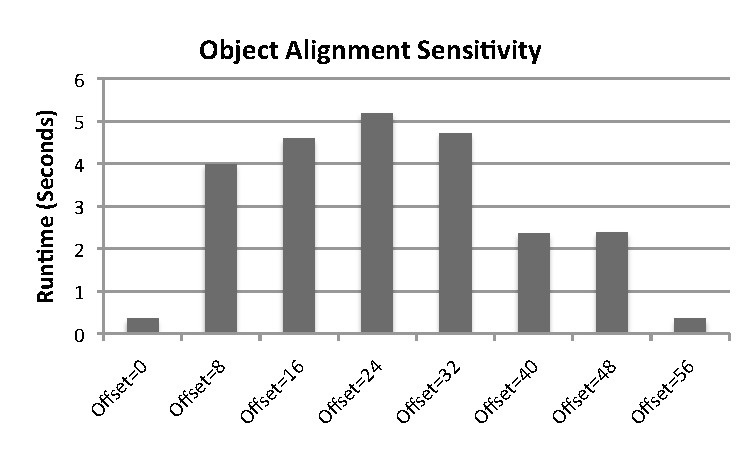
\includegraphics[width=3.3in]{predator/figure/perfsensitive}
\end{center}
\caption{
Performance of the linear\_regression benchmark from the Phoenix benchmark suite.
Performance is highly sensitive to the offset of the starting address of the (potentially) falsely-shared object 
and the start of cache line. 
\label{fig:perfsensitive}}
\end{figure}

The appearance of false sharing depends on 
the alignment between objects and corresponding cache lines.
A real example, linear\_regression, is shown in Figure~\ref{fig:perfsensitive}.
For this benchmark,
when the offset of the starting address between the potentially falsely-shared object and corresponding cache lines 
is $0$ or $56$ bytes, 
there is no false sharing. 
When the offset is $24$ bytes, we see the most severe performance effect caused 
by false sharing. 
The performance difference between these two scenarios can be as large as $15\times$. 
Existing detection tools can only report observed false sharing.
For this case, they may miss a very severe false sharing problem that could occur in the wild if the offset of the starting 
address was $0$ bytes or $56$ bytes in their test environment.
\Predator{} overcomes this shortcoming by accurately predicting potential false sharing.

\begin{figure*}
\begin{center} 
\subfigure[No false sharing]{%
   \label{fig:nofs}
   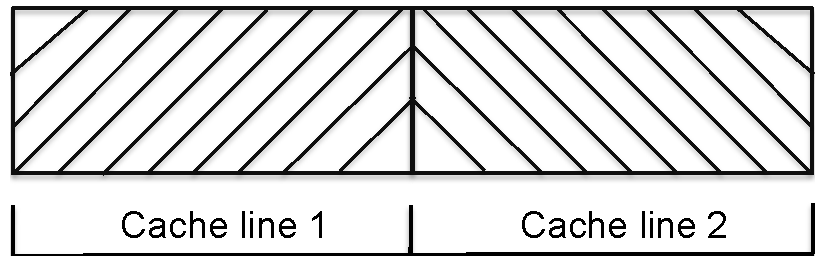
\includegraphics[width=0.24\textwidth]{predator/figure/Potential1}
}%
\hspace{30pt}
\subfigure[False sharing with larger cache size]{%
   \label{fig:fslarger}
   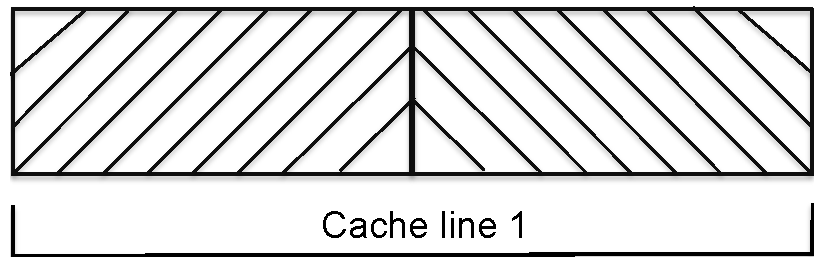
\includegraphics[width=0.24\textwidth]{predator/figure/Potential2}
}%
\hspace{30pt}
\subfigure[False sharing with different alignment]{%
   \label{fig:fsnoalignment}
   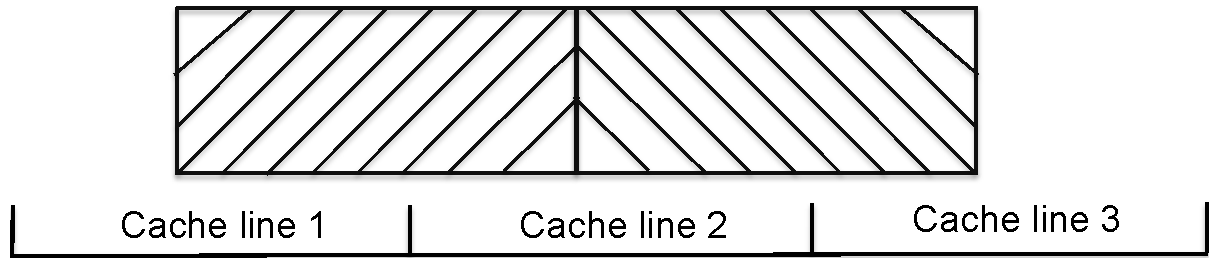
\includegraphics[width=0.36\textwidth]{predator/figure/Potential3}
}%
\end{center}
%\includegraphics{fig/potential.pdf}
\caption{False sharing under different environments.}
\label{fig:potentialfalsesharing}
\end{figure*}

\Predator{} predicts {\it potential false sharing}, the type of
false sharing that does not 
manifest in the current execution but may appear and greatly affect programs' performance
in a slightly different environment.

Figure~\ref{fig:potentialfalsesharing} shows a simplified example why occurrences of false sharing 
can change in different situations.
In this figure, two rectangles with different patterns
represents two portions of the same object, updated by different threads. 
In Figure~\ref{fig:nofs}), there is no false sharing when thread T1 only updates 
``cache line 1'' and T2 only updates ``cache line 2''.
However, false sharing appears in one of the following cases, even with the same
access pattern. 

\begin{itemize}
\item
Doubling cache line size (Figure~\ref{fig:fslarger}). When the size of a
cache line doubles,
both T1 and T2 access the same cache line and false sharing occurs in this case.

\item
Different starting address of an object(Figure~\ref{fig:fsnoalignment}). 
When the starting address of this object is not aligned with the starting address of 
the first cache line, 
then T1 and T2 can update the second cache line simultaneously, 
causing false sharing. 
%When some dynamic property changes the starting address of this object so that it 
%is not aligned with the starting address of the first cache line, 
\end{itemize} 

\Predator{} predicts whether programs can have potential false sharing  
in either of these two cases, where they can be caused by different dynamic properties 
discussed in Section~\ref{sec:intro}.
All dynamic properties, except the change of cache line size,
can lead to different starting address of an object. 
Thus, predicting false sharing in these two cases actually 
explores many possibilities caused by all dynamic properties.

\subsection{Basic Prediction Workflow}
\label{sec:predictionmechanism} 

%Similar to the detection part, 
\Predator{} focuses exclusively on potential false sharing that can 
cause performance problems.
The implementation is based on
two key observations. First, only accesses to 
adjacent cache lines can form potential false sharing, 
i.e., introducing cache invalidations when cache line size
or an object's starting address changes.
Second, only when false sharing introduces a large number of cache invalidations
can it degrade performance.

Based on these two observations, \Predator{} develops 
the following workflow to capture potential false sharing.
Those detection optimizations listed in Section~\ref{optimization} can also be applied
to prediction part. We do not repeat these optimizations in this section.

\begin{enumerate}
\item
Track the number of writes on different cache lines. 

\item
When the number of writes to a cache line $L$ reaches {\it Tracking-Threshold},
track the detailed read and write accesses for every word on both cache line $L$ 
and its adjacent cache lines. 

\item
When the number of writes to a cache line $L$ reaches a second threshold (called as
{\it Predicting-Threshold}), 
identify whether there exists false sharing in $L$ and its adjacent 
cache lines by analyzing word accesses information collected in Step 2. 
Section ~\ref{sec:evaluatingfs} describes the evaluation method.

\item
If a potential false sharing is found, continue to track cache line invalidations to confirm it. Section~\ref{sec:tracking} discusses the details.
Otherwise, go back to Step 2 to track more detailed accesses.
 
\end{enumerate}

\subsection{Searching for Potential False Sharing}
\label{sec:evaluatingfs}
To describe potential false sharing in two different cases, we first 
introduce the concept of a virtual cache line.  A virtual cache line
is a contiguous memory range that spans one or more physical cache 
lines.  In the case of double cache line size, a virtual line is
composed of two original contiguous cache lines and the first cache
line has an even index number.  Thus, only cache lines $2*i$ and
$2*i+1$ can form a virtual line.  In the case of different starting
addresses, a virtual line can have the same size as physical lines,
but can be positioned arbitrarily: unlike actual cache lines, the
starting address of a virtual cache line does not need to be multiple
of the cache line size.  For instance, a 64-byte long virtual line can
consist of the range $[0,64)$ bytes or $[8,72)$ bytes.

To search for potential false sharing problems, 
\Predator{} searches for a hot access pair on $L$ and its adjacent cache lines 
by analyzing the detailed word access information collected in Step 2. 
A hot access in a cache line refers to the word whose number of read or write accesses 
is larger than the average number of accesses to each word of cache line $L$.
For every hot access $X$ in cache line $L$, \Predator{} searches another
hot access $Y$ in $L$'s previous cache line or next cache line satisfying
the following conditions: 

\begin{itemize}
\item
$X$ and $Y$ reside on the same virtual line. 

\item
One of $X$ and $Y$ is a write access.

\item 
$X$ and $Y$ are issued by different threads.

\end{itemize}

% why it finds a pair of $X$ and $Y$ == a potential false sharing 
Whenever it finds such a pair $X$ and $Y$, 
\Predator{} identifies potential performance-degrading false sharing whenever
 the number of cache invalidations caused by $X$ and $Y$, at a possible virtual line, 
is larger than the average number of accesses on each word of $L$. 
This approach is based on a similar observation as in detection:
\emph{if a thread writes a virtual line after other threads 
have accessed the same virtual line, this write operation most likely causes at least one cache 
invalidation}. 
Before tracking detailed memory accesses on a virtual line, it is impossible to know exactly how many cache invalidations happen on a virtual line. Thus, \Predator{} conservatively assumes that accesses from different threads occurs interleavedly.
This approach ensures that \Predator{} does not miss any potential false sharing as well as 
not reporting false positives. 

%According to above observation and assumption, 
%a pair of hot accesses, $X$ and $Y$, if accesses are issued in an interleaving 
%way, can generate the number of cache invalidations equaling to 
%the smaller number of accesses of $X$ and $Y$.
%Thus a false sharing problem is to be identified by \Predator{}.
  
After identifying possible false sharing, \Predator{} goes to Step 4 to 
verify whether this is an actual false sharing problem.

\subsection{Verifying Potential False Sharing}
\label{sec:tracking}

\Predator{} verifies potential false sharing by tracking 
cache invalidations on a problematic virtual line.
%covering a pair of hot accesses found
%in Step 3.

For potential false sharing caused by double cache line size, as described in
Section~\ref{sec:evaluatingfs}, a virtual line is always composed of 
cache line with index $2*i$ and $2*i+1$. 
\Predator{} tracks cache invalidations
on the virtual line on which false sharing has been discovered.

However, for the case of a change in starting address,
two hot accesses with distance less than cache line size 
can form multiple virtual lines. 
There is thus an additional step to determine which virtual line to be tracked.
Although the virtual line to be chosen here is never a real cache line of actual hardware
because of unaligned addresses,
we utilize this virtual line to simulate the effect of changing the 
starting addresses of objects.


\begin{figure}
\begin{center} 
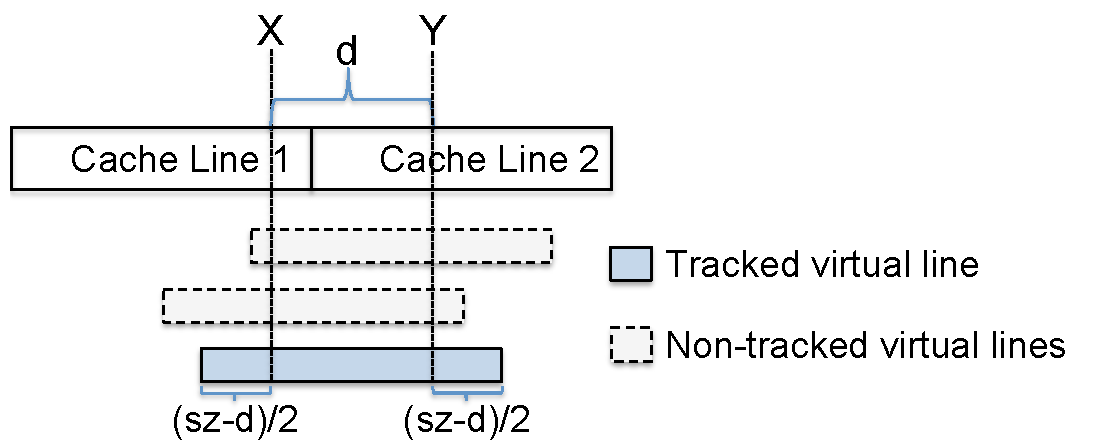
\includegraphics[width=3.3in]{predator/figure/trackpotential}
\end{center}
\caption{Determining a virtual line with size $sz$ according to hot accesses.}
\label{fig:trackpotential}
\end{figure}

Given two words with the hot accesses shown in Figure~\ref{fig:trackpotential}, 
\Predator{} leaves the same space before $X$ and after $Y$ in determining a virtual line. 
That is, the virtual line starting 
at location $X-((sz-d)/2)$ and ending at $Y+((sz-d)/2)$ is tracked. 
This choice allows tracking of more possible cache invalidations caused by
adjacent accesses of $X$ and $Y$. 
Since adjusting the starting address of a virtual line has the same effect of
adjusting the starting address of an object in detecting false sharing,
all cache lines related to the same object must be adjusted at the same time.
\Predator{} then tracks cache invalidations based on these adjusted virtual lines.



\section{Evaluation}
\begin{figure*}[htb]
{\centering
\tiny
\subfigure{\lstinputlisting[numbers=none,frame=none,boxpos=t]{predator/figure/linearregression.report}}
\caption{An example report by \Predator{} indicating false sharing in the linear\_regression benchmark.
\label{fig:lrreport}}
}
\end{figure*}



\label{sec:evaluation}

This section answers the following questions:
\begin{itemize}
\item
  How effective is \Predator{} at detecting and predicting false sharing?

\item
  What is \Predator{}'s overhead, in terms of execution time and memory ?

\item
  How sensitive is \Predator{} to different sampling rates?
 
\end{itemize}

\paragraph{Experimental Platform.} All evaluations are performed on a quiescent Intel Core 2 dual-processor system equipped with 
16GB RAM. Each processor is a 4-core 64-bit Intel Xeon running at 2.33 GHz, with a 4MB shared L2 cache and 32KB private L1 cache. The underlying operating system is an unmodified CentOS 5.5, running with Linux kernel version 2.6.18-194.17.1.el5. The glibc version is 2.5. 

\paragraph{Evaluated Applications.}
This paper evaluates two popular benchmark suites,
Phoenix (with large input) ~\cite{phoenix-hpca} and PARSEC (with simlarge input) ~\cite{parsec}. Even with unmodified LLVM-3.2, Facesim cannot be compiled successfully (having complaints on an undefined template) and Canneal aborts unexpectedly. Thus, these two benchmarks are excluded.
We also evaluate \Predator{} on six real applications, including MySQL, Boost, Memcached, aget, pbzip2 and pfscan.



\subsection{Detection and Prediction Effectiveness}
\label{sec:effective}

For every false sharing problem, \Predator{} reports source code information and detailed memory access information in order to help users fix those problems. Figure~\ref{fig:lrreport} shows an example for the linear\_regression benchmark. This report shows that the heap object starting with $0x40000038$ potentially causes a large number of cache invalidations. The call stack of allocation is provided to help locate culprits. In addition, \Predator{} also reports word-level access information of this object, which helps to identify where and how false sharing occurs. From that, we can know that it is a latent false sharing problem predicted by \Predator{}, since different threads are accessing different cache lines. 

\subsubsection{Benchmarks}
\label{sec:benchmarks}

\begin{table*}[!t]
{\centering\begin{tabular}{l|r|r|r|r|r}\hline
{\bf \small Benchmark} & {\bf \small Source Code} & {\bf \small New} & {\bf \small Without Prediction} &{\bf \small With Prediction} & {\bf \small Improvement} \\
\hline
\small \textbf{histogram} & {\small histogram-pthread.c:213} & \cmark{} &\cmark{} & \cmark{} & 46.22\%\\
\small \textbf{linear\_regression} & {\small linear\_regression-pthread.c:133} & & & \cmark{} & 1206.93\% \\
\small \textbf{reverse\_index} & {\small reverseindex-pthread.c:511} & & \cmark{} & \cmark{} & 0.09\%\\
\small \textbf{word\_count} & {\small word\_count-pthread.c:136} & & \cmark{} & \cmark{} & 0.14\%\\
\hline
\small \textbf{streamcluster} & {\small streamcluster.cpp:985} &  & \cmark{} & \cmark{} &7.52\% \\
\small \textbf{streamcluster} & {\small streamcluster.cpp:1907} & \cmark{} & \cmark{} & \cmark{} & 4.77\%\\
\hline
\end{tabular}
\caption{False sharing problems in the Phoenix and PARSEC benchmark suites. \label{table:detection}}
}
\end{table*}

Table~\ref{table:detection} provides detection results of two benchmark suites, Phoenix and PARSEC
The first column lists those programs with false sharing problems.  The second column shows precisely where the problem is. Because all discovered false sharing occurs inside heap objects, we show callsite source code information here.  The third column, ``New'', marks whether this false sharing was newly discovered by \Predator{}.  A checkmark in the following two columns indicates whether the false sharing was identified without
prediction and/or with prediction.  The final column, ``Improvement'', shows the performance improvement after fixing false sharing.
%The number is based on the average runtime of $10$ runs. 

As shown in the table, \Predator{} reveals two unknown false sharing problems. It is the first tool to detect the false sharing problems in histogram and in line $1908$ of streamcluster. 
In histogram, multiple threads simultaneously modify different locations of the same heap object, thread\_arg\_t. 
Padding this data structure fixes the false sharing problem and improves the performance by around 46\%. In streamcluster, multiple threads are simultaneously accessing and updating the same \texttt{bool} array, switch\_membership. Simply changing all elements of this array to a long type reduces the false sharing and improves the performance by about 4.7\%.

%, although it is not a complete fix of false sharing. 
%None of these two false sharing problems has been reported by previous tools.
Other false sharing problems were discovered by previous work~\cite{sheriff}. We do not see significant performance improvement for reverse\_index and word\_count benchmarks. They are reported here because the number of cache invalidations in these two programs reaches our predefined threshold.
Making the reporting threshold higher can avoid the report of those insignificant false sharing problems.
It is worth noting that these two benchmarks definitely have false sharing problems,
which can be confirmed by word-level information generated by \Predator{}. 

The streamcluster benchmark has another false sharing problem at line $985$. Different threads change the work\_mem object simultaneously. Authors of streamclsuter have already realized this problem and provide a CACHE\_LINE macro. Unfortunately, the default value of this macro is set to $32$ bytes, which is different from the actual cache line size of the experimental machine. By setting it to $64$ bytes instead, it achieves  performance improvement of about 7.5\%.

linear\_regression has a severe false sharing problem. Fixing it improves the performance by more than $12\times$. In this benchmark, different threads update their thread-specific locations inside the tid\_args object in a tight loop. According to the observation of Nanavati et al., this false sharing problem occurs when using clang and disappears when using gcc with the -O2 and -O3 optimization level~\cite{OSdetection}. But we observed a different result when using the clang-3.2 compiler and our custom memory allocator: the false sharing problem does not occur at all because the offset of the starting address of the potentially falsely-shared object and the start of cache line is 56 bytes (see Figure~\ref{fig:perfsensitive}). With prediction mechanism, \Predator{} detects this latent false sharing problem, exemplifying the necessity of a predictive detection tool. 

\subsubsection{Real Applications}
To verify \Predator{}'s practicality, we further evaluate several widely-used real applications, whereas no previous work has done this. These real applications include a server application (MySQL~\cite{mysql}),
a standard C++ library (Boost~\cite{libfalsesharing}),
a distributed memory object caching system (Memcached), a network retriever (aget),
a parallel bzip2 file compressor (pbzip2), and a parallel file scanner (pfscan).

MySQL-5.5.32 and boost-1.49.0 are known to have false sharing problems. Other applications (memcached-1.4.15, aget-0.4.1 and pbzip2-1.1.6) do not have known false sharing problems.

The false sharing of MySQL has caused a significant scalability problem and was very difficult to identify.
According to the architect of MySQL, Mikael Ronstrom, ``we had gathered specialists on InnoDB..., participants from MySQL support... and a number of generic specialists on 
computer performance...'', ``[we] were able to improve MySQL performance by 6$\times$ with those scalability fixes''~\cite{mysql}. 
The false sharing inside Boost is caused by the usage of a  spinlock pool. Different threads may utilize different spinlocks located in the same cache line in this case. Fixing it brings a 40\% performance improvement.
\Predator{} is able to pinpoint false sharing locations in both MySQL and the Boost library. 
For the other four applications, \Predator{} does not find severe false sharing problems.

\subsubsection{Prediction Effectiveness}
\label{sec:predicteval}
In this section, we verify whether prediction can always  reveal un-observed false sharing problems.

The linear\_regression benchmark is selected here because of the following two reasons: (1) The false sharing problem of this benchmark cannot be detected without prediction; (2) False sharing severely degrades performance when it actually occurs. Hence, it is a serious problem that should always be detected. 

\begin{figure}[!t]
{\centering
\subfigure{\lstinputlisting[numbers=none,frame=none,boxpos=t]{predator/figure/linearregression.psedocode}}
\caption{The false sharing problem inside the linear\_regression benchmark: multiple threads simultaneously update their entries in lreg\_args.
\label{fig:linearregression}}
}
\end{figure}

Figure~\ref{fig:linearregression} shows the data structure and the source code exercising appropriate false sharing. The size of this data structure, lreg\_args, is $64$ bytes 
when the program is compiled to a $64$-bit binary. For this benchmark, the main thread allocates an array, containing as many elements as the number of underlying hardware cores. Each element is a lreg\_args type with $64$ bytes. This array is then passed to different threads (lreg\_thread function) so that each thread only updates its thread-dependent area. False sharing occurs if two threads happen to update data in the same cache line. 

Figure~\ref{fig:perfsensitive} shows how sensitive the performance is to different starting addresses of a falsely-shared object. When the offset is $0$ or $56$ bytes, this benchmark achieves its optimal performance and has no false sharing. When the offset is $24$ bytes, the benchmark runs around $15$ times slower than its optimal performance because of the false sharing problem.

Our evaluation shows that \Predator{} can always detect the false sharing problem with prediction enabled, demonstrating its effectiveness.

\subsection{Performance Overhead}
\label{sec:perfoverhead}

\begin{figure*}[!t]
\centering
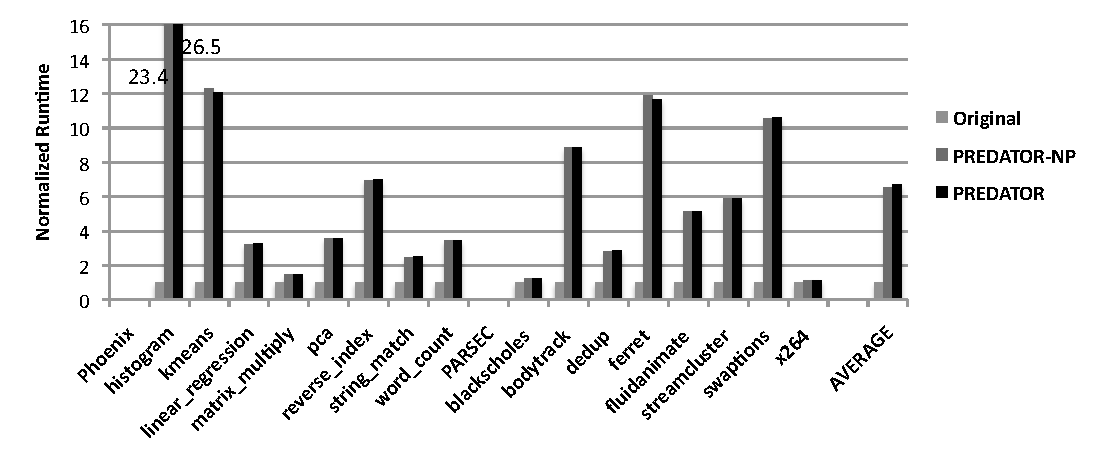
\includegraphics[width=6in]{predator/figure/perf}
\caption{
Performance overhead of \Predator{} with and without prediction(PREDATOR-NP).
\label{fig:perf}}
\end{figure*}

To avoid the effect caused by extreme outliers, all performance data shown in Figure~\ref{fig:perf} is based on the average of $10$ runs, excluding the maximum and minimum values. 

For $16$ benchmarks from the Phoenix and PARSEC benchmark suites and six real applications, \Predator{} imposes $5.4\times$ performance overhead. There is no noticeable difference on performance whether the prediction mechanism is enabled or not. 
 
Among these programs, five of them, histogram, kmeans, bodytrack, ferret, and swaptions, have more than $8\times$ performance overhead. The histogram benchmark runs more than $26\times$ slower than original executions with \pthreads{} library, because tracking detailed access on cache lines with false sharing exacerbates the false sharing effect (see more discussion in Section~\ref{sec:sample}).  For bodytrack and ferret, although there is no false sharing, \Predator{} detects a large amount of cache lines with writes larger than {\it Tracking-Threshold}. Thus, tracking those accessing details for those cache lines imposes significant performance overhead. Currently, we cannot identify the reasons why kmeans runs very slowly on \Predator{}.
   
\Predator{} imposes a small performance overhead for IO-bound applications, such as matrix\_multiply, blackscholes, x264, aget, Memcached, pbzip2, and pfscan, since \Predator{} does not add any performance overhead for IO operations.  

\subsection{Memory Overhead}
\label{sec:memoverhead}
We only evaluate the physical memory overhead of \Predator{}, instead of the virtual memory overhead, because \Predator{} allocates four gigabytes virtual memory for its custom memory allocator. Proportional set size (PSS) in \texttt{/proc/self/smaps} reflects the physical memory increase on the existing system of running an application~\cite{memusage}. Thus, we periodically collect this data and use the sum of different memory mappings as the total physical memory usage of running an application. We present the maximum value of physical memory usage in Figure~\ref{fig:memusage}. 

\Predator{} imposes less than 50\% memory overhead for 17 out of 22 applications.  For swaptions and aget, \Predator{} introduces more memory overhead because the original memory footprints of them are very small, only $3$ kilobytes. Adding the code of detection, prediction and reporting contributes to a large ratio of memory overhead. We are not clear why MySQL consumes much more memory than others. Although the average memory usage of all applications is over $2\times$, the total memory usage overhead is only about $40\%$ on \Predator{}. 


\subsection{Sensitivity to Different Sampling Rates}
\label{sec:sensitivity}
In Section~\ref{sec:sample}, we discuss that \Predator{} utilizes the sampling mechanism to reduce the tracking overhead. Running an application with different sampling rates does not affect its memory usage. Thus, we only evaluate the effect of different sampling rates on performance and effectiveness. 

The default sampling rate used by \Predator{} is 1\%. In this section, we also evaluate two other sampling rates, 0.1\% and 10\%. The performance results under the three different sample rates are shown in Figure~\ref{predator/figure:sample}. \Predator{} introduces less performance overhead under a lower sampling rate, which meets our expectation. Concerning effectiveness, even using the 0.1\% sampling rate, \Predator{} can still detect all false sharing problems, but with a lower number of cache invalidations. Thus, different sampling rates do not affect the detection effectiveness.
 
\begin{figure*}[!t]
\centering
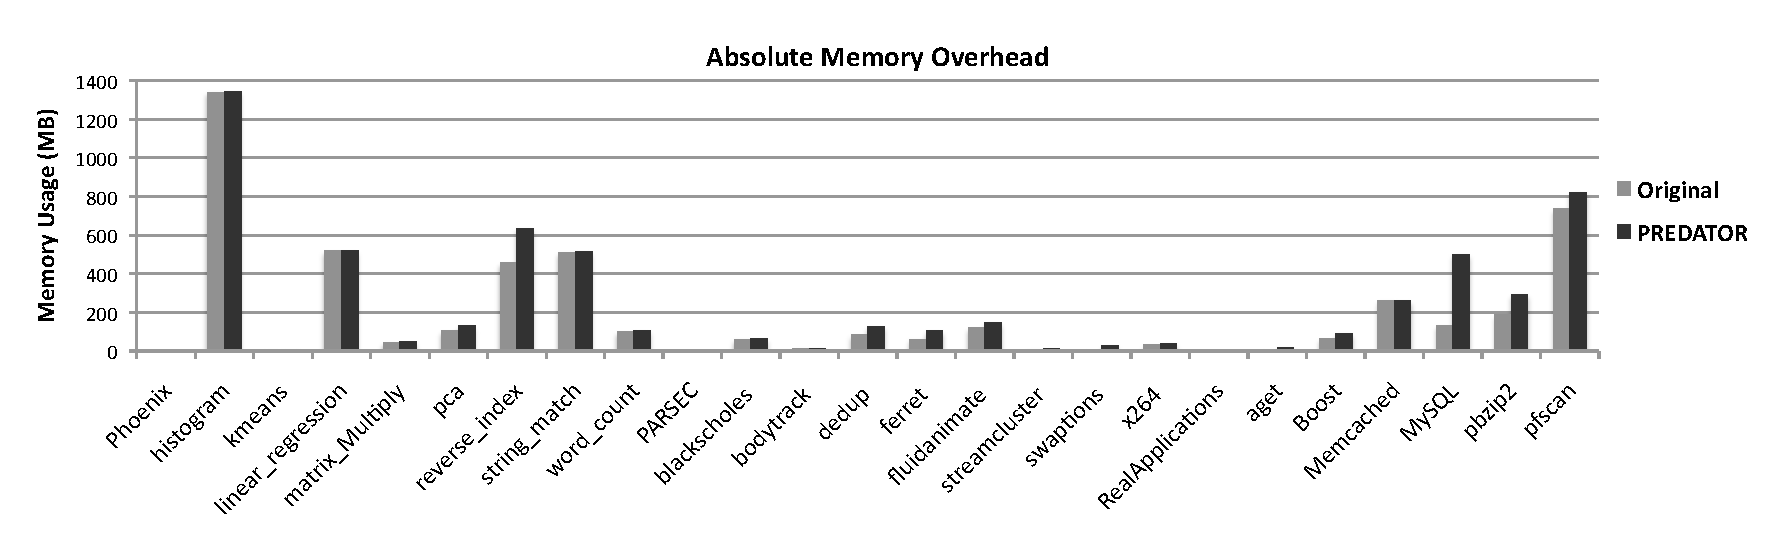
\includegraphics[width=6in]{predator/figure/absolutememory}
\caption{Absolute physical memory usage overhead with \Predator{}.}
\label{fig:absolutememusage}
\end{figure*}

\begin{figure*}[!t]
\centering
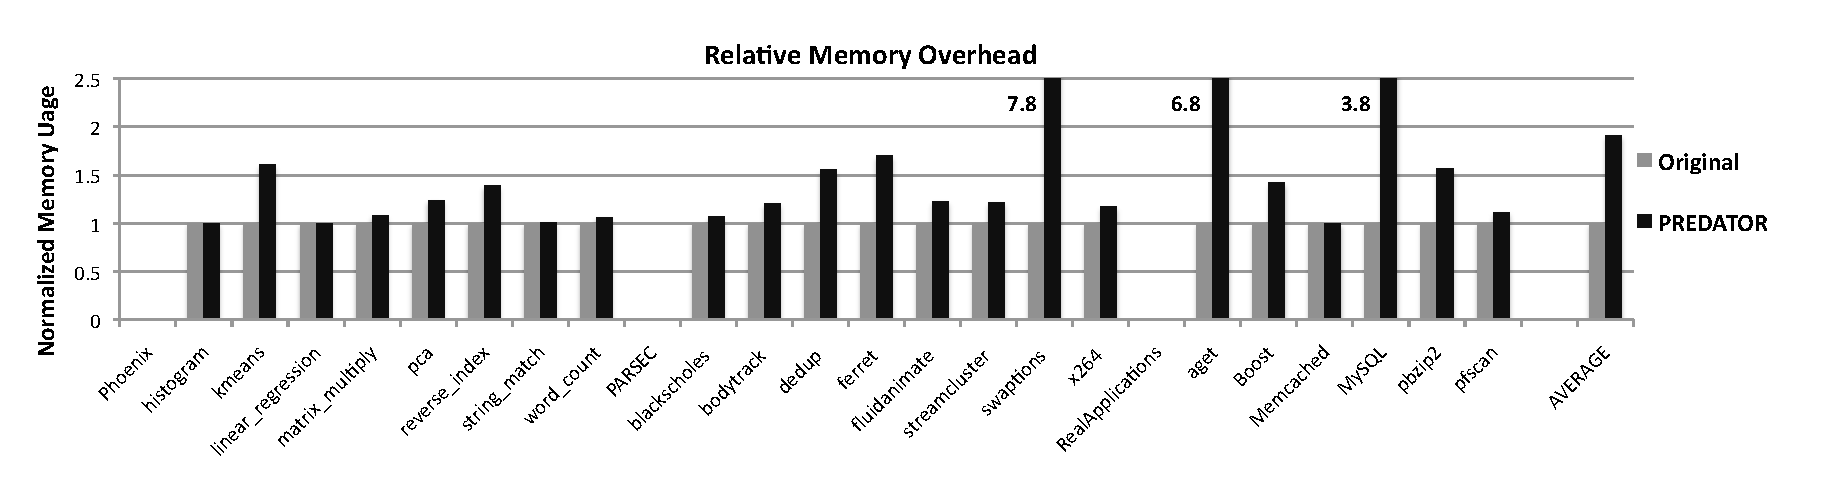
\includegraphics[width=6in]{predator/figure/memusage}
\caption{Relative physical memory usage overhead with \Predator{}.}
\label{fig:memusage}
\end{figure*}




